\documentclass[border=10pt]{standalone}

\usepackage{tikz}
\usepackage{tikzsymbols}
\usetikzlibrary{calc,patterns,shapes.geometric}

\def\centerarc[#1](#2)(#3:#4:#5){\draw[#1] ($(#2)+({#5*cos(#3)},{#5*sin(#3)})$) arc (#3:#4:#5);}

\begin{document}
	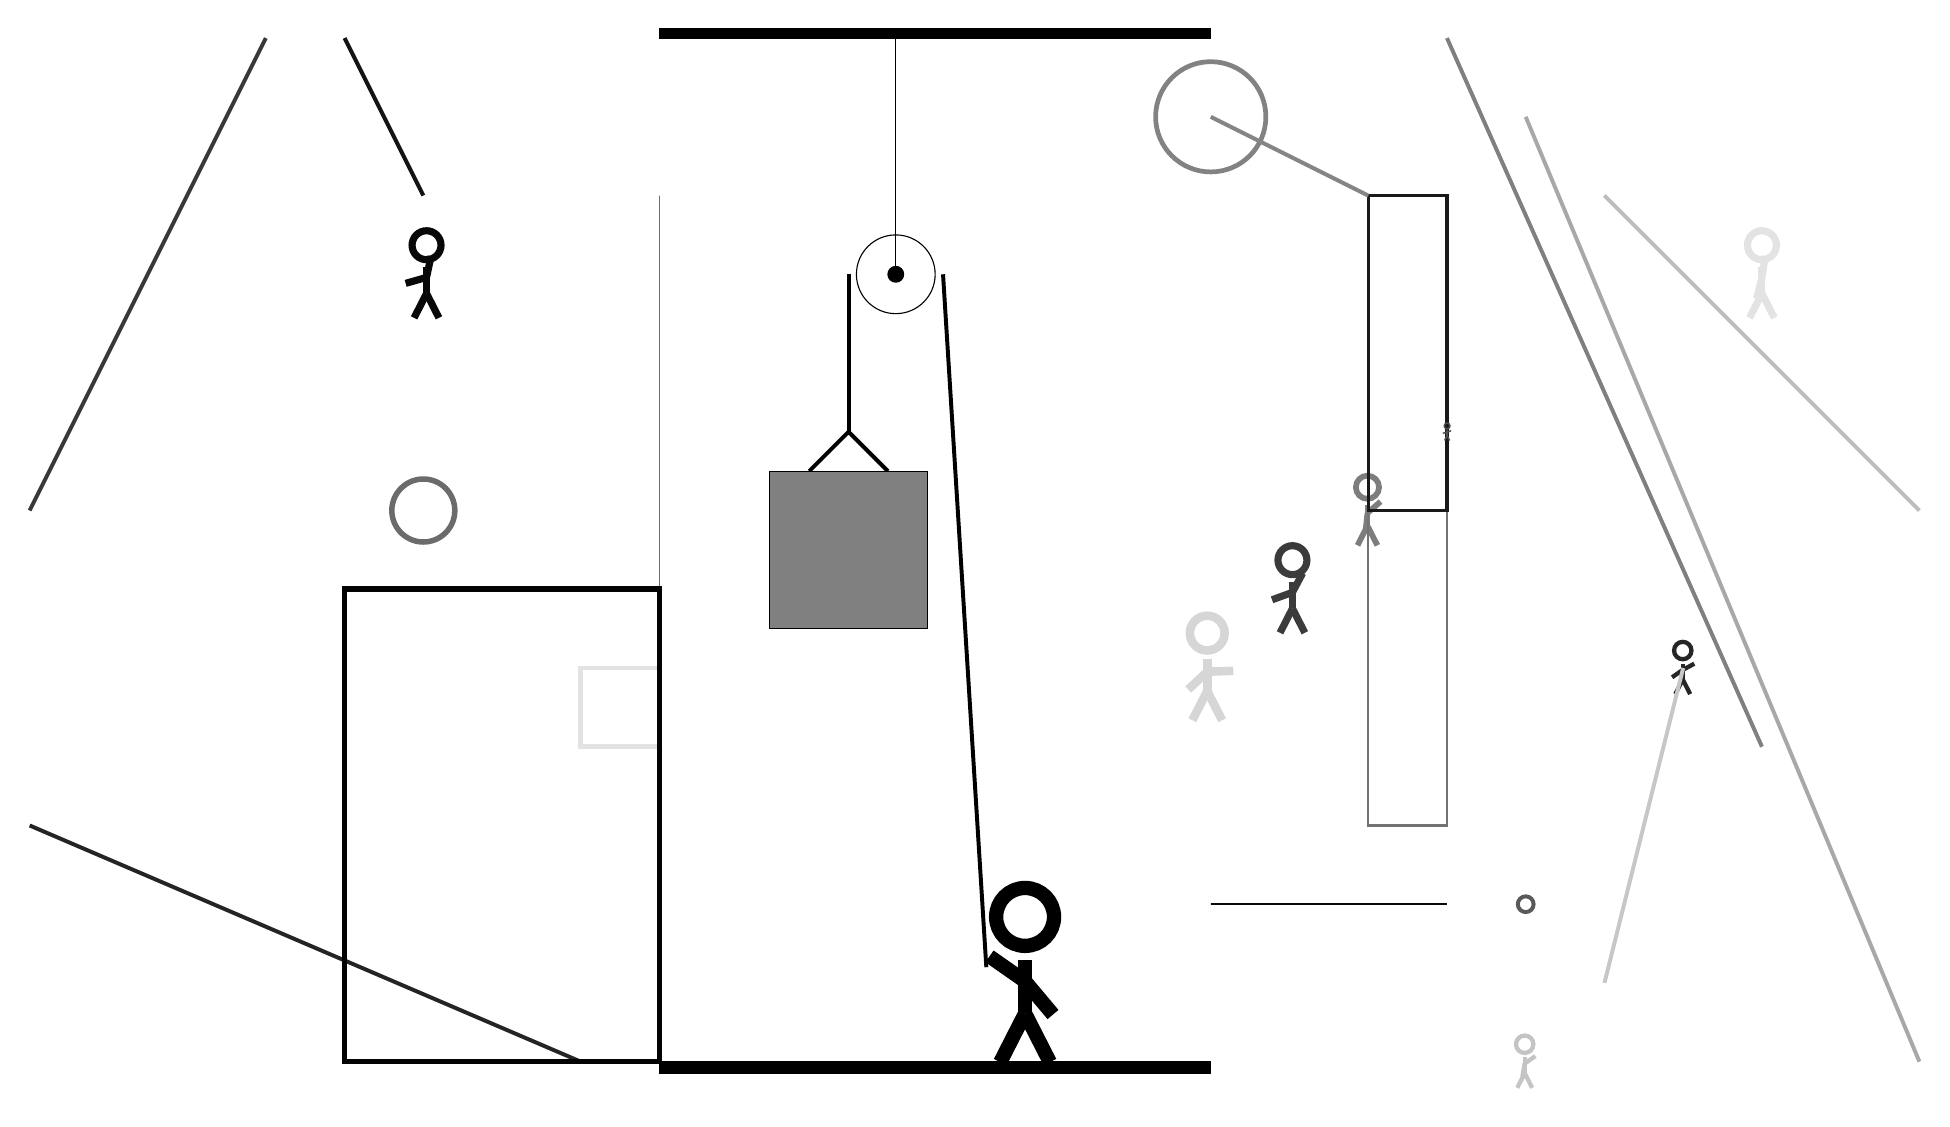
\begin{tikzpicture}
		%%%%% START %%%%%
		
		\draw[fill=black] (-2, 10) rectangle (5, 10.125);
		
		\draw (1, 7) circle (0.5);
		\draw[fill=black] (1, 7) circle (0.1);
		\draw (1, 10) -- (1, 7);
		
		\draw[line width=0.5mm] (-0.1, 4.5) -- (0.4, 5.0) -- (0.9, 4.5);
		\draw[fill=black!50] (-0.6, 4.5) rectangle (1.4, 2.5);
		
		\node[line width=0.3mm, color=black!11] at (12, 7) {\Strichmaxerl[5][76][81]};
		
		\draw[line width=0.5mm, color=black!50](8, 10) -- (12, 1);
		\node[line width=0.5mm, color=black!51] at (7, 4) {\Strichmaxerl[4][84][41]};
		\draw [line width=0.7mm, color=black!58](-5, 4) circle (0.4);
		
		\draw[line width=0.3mm, color=black!55] (7, 0) rectangle (8, 8);
		\draw[line width=0.5mm, color=black!92](-5, 8) -- (-6, 10);
		\draw[line width=0.5mm, color=black!86](-3, -3) -- (-10, 0);
		
		\draw[line width=0.4mm, color=black!90] (7, 8) rectangle (8, 4);
		\draw[line width=0.5mm, color=black!94](-6, -2) -- (-6, -2);
		\node[line width=0.3mm, color=black!97] at (-5, 7) {\Strichmaxerl[5][16][78]};
		
		\draw [line width=0.6mm, color=black!61](-3, 6) circle (0.0);
		
		\draw[line width=0.5mm, color=black!78](-7, 10) -- (-10, 4);
		\draw [line width=0.6mm, color=black!49](5, 9) circle (0.7);
		
		\draw [line width=0.6mm, color=black!38](-4, 7) circle (0.0);
		\node[line width=0.4mm, color=black!16] at (5, 2) {\Strichmaxerl[6][43][2]};
		\node[line width=0.6mm, color=black!85] at (11, 2) {\Strichmaxerl[3][35][28]};
		
		\draw[line width=0.5mm, color=black!26](10, 8) -- (14, 4);
		\draw[line width=0.2mm, color=black!57] (-2, 8) rectangle (-2, -3);
		\draw[line width=0.6mm, color=black!11] (-3, 1) rectangle (-2, 2);
		\draw[line width=0.5mm, color=black!22](10, -2) -- (11, 2);
		\draw [line width=0.5mm, color=black!65](9, -1) circle (0.1);
		
		\node[line width=0.7mm, color=black!23] at (9, -3) {\Strichmaxerl[3][80][35]};
		\node[line width=0.7mm, color=black!77] at (6, 3) {\Strichmaxerl[5][20][62]};
		\node[line width=0.2mm, color=black!69] at (8, 5) {\Strichmaxerl[1][10][24]};
		\draw[line width=0.7mm, color=black!99] (-2, 3) rectangle (-6, -3);
		
		\draw[line width=0.5mm, color=black!48](5, 9) -- (7, 8);
		\draw[line width=0.3mm, color=black!96] (5, -1) rectangle (8, -1);
		\draw[line width=0.5mm, color=black!34](9, 9) -- (14, -3);
		
		
		\draw[line width=0.5mm] (0.4, 7) -- (0.4, 5.0);
		\centerarc[line width=0.5mm](1, 7)(0:180:0.6);
		\draw[line width=0.5mm](1.6, 7) -- (2.15, -1.8);
		
		\node at (2.6, -1.9) {\Strichmaxerl[10][-35][-50]};
		
		\draw[fill=black] (-2, -3) rectangle (5, -3.15);
		
		%%%%% END %%%%%
	\end{tikzpicture}
\end{document}